\documentclass[../gruppenarbeit_1.tex]{subfiles}
  
\subsection{Einführung}

Die Logik formalisiert wie man über etwas exakt spricht, denkt und 
kommuniziert. Damit werden die Themen worüber man spricht, präzisiert
und unzweideutig formalisiert. Dies ist auch bekannt als
"\textbf{formale Wissenschaft}".

\begin{align}
\fbox{\begin{minipage}{11.8cm}
  \textbf{Beispiel}: Ein Computer-Chip Hersteller benötigt klare, formale 
  Spezifikationen (Logik) für seine Produkte, bevor die Hardware in 
  die Herstellung gelangt. Ansonsten werden Fehler sehr kostspielig.
\end{minipage}}
\end{align}

Somit bezeichnen wir eine logische Aussage als Satz, der entweder
\textbf{wahr} (true) oder \textbf{falsch} (false) ausdrückt. Dabei 
unterscheiden wir die \textbf{Elementaraussage} (oder auch atomare 
Aussage/Formel) und die \textbf{zusammengesetzte Aussage}, welche sich aus
einzelnen Teilaussagen zusammen setzt.

\begin{align}
\fbox{\begin{minipage}{11.8cm}
  \textbf{Hinweis}: In der Logik/Informatik gibt es Probleme, die keine
  aussagen kräftige Antworten haben. Man weiss also nicht, ob es
  entscheidbar/beweisbar ist.
\end{minipage}}
\end{align}

Beispiele von logischen Aussagen:

\begin{itemize}
  \item Es ist gerade 15 Grad (wahr)
  \item Die Erde ist flach (falsch)
  \item 4 plus 4 ist 8 (wahr)
  \item x ist eine ungerade Zahl\\
        \textbf{Achtung}: dies ist eine Aussagenform aber keine Aussage)
\end{itemize}

Weitere Definitionen:

\begin{itemize}
  \item \textbf{Atomare Aussage}\\
        $A$ $\arrowvert$ ein enzelnes (kleinstes) Element
  \item \textbf{Atomare Formel}\\
        $Var = { A, B, C }$, Ansammlung atomarer Aussagen
  \item \textbf{Induktion}\\
        $Var = { A, B, C } = f$, Als Zusammenfassung, daraus: $\lnot f$
  \item \textbf{Gesamtheiten}\\
        $F_{AL}$, Gesamtheit aller aussagenlogischer Formeln\\
        $Var(f)$, Gesamtheit aller atomaren Formeln einer aussagenlogischen 
        Formel
  \item \textbf{Literal} ist eine atomare Formel oder deren Negation
\end{itemize}

\newpage

\subsection{Konnektoren, Junktoren und Operatoren}

\def\arraystretch{1.5}
\begin{table}[ht]
\begin{tabular}[t]{ll}
\hline
  Kürzel & Definition\\
\hline
  $A, B$ & Variabeln\\
  $\land$ & Konjunktion, logisches UND\\
  $\lor$ & Disjunktion, logisches ODER\\
  $\lnot$A oder $\bar{A}$ & Negation\\
  $\Rightarrow$ & Implikation ($A$ = Prämisse, $B$ = Konklusion)\\
  $\iff$ & Äquivalenz\\
\hline
\end{tabular}
\end{table}

Dabei gilt die folgende Bindungsstärke:

\begin{enumerate}
  \item $\lnot$ \hspace{11.5mm} Negation
  \item $\land$ $\lor$ \hspace{8mm} Konjunktion \& Disjunktion
  \item $\Rightarrow$ $\iff$ \hspace{1mm} Implikation \& Äquivalenz
\end{enumerate}

Wenn wir diese Regeln verletzen, müssen wir das gewünschte Ergebnis
mit einer Klammer $()$ kennzeichnen.

\subsubsection{Konjunktion, Disjunktion und Negation}

Nachfolgend stellen wir die Wahrheitstabellen der Konjunktion,
Disjunktion und Negation anhand von $A$ und $B$ dar:

\begin{table}[ht]
\begin{tabular}{c|c||c}
  A & B & A $\land$ B \\ \hline
  0 & 0 & 0 \\
  0 & 1 & 0 \\
  1 & 0 & 0 \\
  1 & 1 & 1 \\
\end{tabular}
\quad
\begin{tabular}{c|c||c}
  A & B & A $\lor$ B \\ \hline
  0 & 0 & 0 \\
  0 & 1 & 1 \\
  1 & 0 & 1 \\
  1 & 1 & 1 \\
\end{tabular}
\quad
\begin{tabular}{c|c||c}
  A & B & $\lnot$(A $\lor$ B) \\ \hline
  0 & 0 & 1 \\
  0 & 1 & 0 \\
  1 & 0 & 0 \\
  1 & 1 & 0 \\
\end{tabular}
\end{table}

Die Konjunktion und Disjunktion können wir auch verallgemeinert darstellen:

\vspace{2mm}
Konjunktion:
\hspace{5mm}
$\bigwedge \limits_{i=1}^n A_i := A_1 \land A_2 \land ... \land A_n$ \par
\vspace{2mm}

Disjunktion:
\hspace{6.4mm}
$\bigvee \limits_{i=1}^n A_i := A_1 \lor A_2 \lor ... \lor A_n$ \par

\subsubsection{Äquivalenz, Implikation und deren Negation}

Grundsätzlich können wir mit $\land$, $\lor$ und $\lnot$ alle Fälle der Logik
abdecken. Zusätzlich nutzen wir noch die Definition der Äquivalenz und der
Implikation:

\begin{table}[ht]
\begin{tabular}{c|c||c}
  A & B & A $\iff$ B \\ \hline
  0 & 0 & 1 \\
  0 & 1 & 0 \\
  1 & 0 & 0 \\
  1 & 1 & 1 \\
\end{tabular}
\quad
\begin{tabular}{c|c||c}
  A & B & A $\Rightarrow$ B \\ \hline
  0 & 0 & 1 \\
  0 & 1 & 1 \\
  1 & 0 & 0 \\
  1 & 1 & 1 \\
\end{tabular}
\quad
\begin{tabular}{c|c||c}
  $\lnot$A & $\lnot$B & A $\Rightarrow$ B \\ \hline
  0 & 0 & 1 \\
  0 & 1 & 0 \\
  1 & 0 & 1 \\
  1 & 1 & 1 \\
\end{tabular}
\end{table}

Die Äquivalenz ist selbsterklärend; wenn $A$ gleich ist wie $B$, dann ist die
Aussage \textbf{wahr}. Die Implikation ist etwas komplexer, sie besagt
aus $A$ folgt $B$:

\begin{align}
\fbox{\begin{minipage}{11.8cm}
  \textbf{Beispiel}:\\
  \\
  Als Grundlage nehmen wir die folgende Aussage:\\
  $A \to$ $"$Ich hab Lust auf Pizza$"$ und \\
  $B \to$ $"$Ich gehe einkaufen".\\
  Nun analysieren wir aus $A$ folgt $B$:
  \begin{itemize}
    \item Ich hab Lust auf Pizza (1), also gehe ich einkaufen. (1)
          \\ = \textbf{wahr} (ist eine wahre Aussage)
    \item Ich hab Lust auf Asiatisch (0, da nur wahr, wenn Pizza), \\
          also gehe ich einkaufen. (1)
          \\ = \textbf{wahr} (ist eine wahre Aussage)
    \item Ich hab Lust auf Pizza (1), \\
          bleibe daher zuhause. (0, da nur wahr, wenn einkaufen)
          \\ = \textbf{falsch} (ist eine falsche Aussage, ergibt keinen Sinn)
    \item Ich hab keine Lust auf Pizza (0), also bleibe ich Zuhause (0)
          \\ = \textbf{wahr} (ist eine wahre Aussage, ergibt Sinn)
  \end{itemize}
  Dies lässt sich nun auch logisch auf die Negation der Implikation anwenden.
\end{minipage}}
\end{align}

\newpage

\subsubsection{Exklusive Oder}

Das exklusive Oder ($XOR$) ist die Umkehroperation der Äquivalenz:

\begin{table}[ht]
\begin{tabular}{c|c||c}
  A & B & $A$ $\dot {\lor }$ $B$ \\ \hline
  0 & 0 & 0 \\
  0 & 1 & 1 \\
  1 & 0 & 1 \\
  1 & 1 & 0 \\
\end{tabular}
\quad
\begin{tabular}{l}
  Oft wird auch folgende Schreibweise angewendet:\\
  $XOR := \dot {\lor } := \lnot(A \iff B)$
\end{tabular}
\end{table}

\subsection{Syntax und Semantik}

Die \textbf{Semantik} definiert die Bedeutungslehre, wie ich eine
logische Aussage interpretieren muss. Der \textbf{Syntax} definiert dabei
Regeln, sowie die elementaren Zeichen oder Symbolgruppen.

\subsubsection{Syntax}

Wir fragen uns:

\begin{quotation}
  Ist diese logische Aussage/Formel formal korrekt?
\end{quotation}

ln $f$ und $g$ sind syntaktisch gleich, wenn sie aus der gleichen
Zeichenreihenfolge bestehen. Wir schreiben dann:

\begin{align}
  f = g
\end{align}

Die Syntax kann dabei aus einem sogenannten Ableitungsbaum gelesen werden:

\begin{align}
  f = (A \lor B) \land \lnot C
\end{align}

\begin{align}
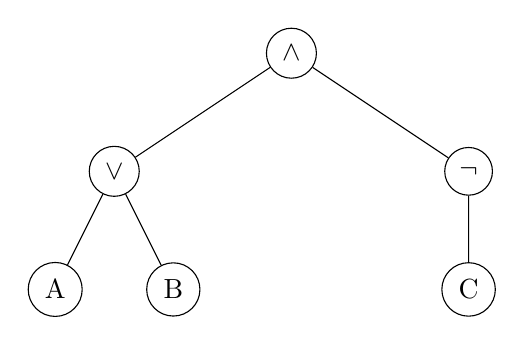
\begin{tikzpicture}[nodes={draw, circle}, -]
\node{$\land$}
  child { node {$\lor$} 
      child { node {A} }
      child { node {B} }
  }
  child [missing]
  child [missing]
  child { node {$\lnot$} 
      child { node {C} }
  };
\end{tikzpicture}
\end{align}

\subsubsection{Semantik}

Wir fragen uns:

\begin{quotation}
  Was bedeutet diese logische Aussage/Formel?
\end{quotation}

Zwei Formeln $f$ und $g$ sind semantisch gleich (Äquivalent), wenn ihre
Wahrheitstabelle identisch sind. Wir schreiben dann:

\begin{align}
  f \equiv g
\end{align}

Neben der Darstellung mithilfe des Ableitungsbaumes können wir ebenfalls die
Wahrheitstabelle nutzen:

\begin{table}[ht]
\begin{tabular}{c|c|c||c}
  A & B & C & $f = (A \lor B) \land \lnot C$ \\ \hline
  0 & 0 & 0 & $(0) \land 1 = \textbf{0}$ \\
  0 & 0 & 1 & $(0) \land 0 = \textbf{0}$ \\
  0 & 1 & 0 & $(1) \land 1 = \textbf{1}$ \\
  0 & 1 & 1 & $(1) \land 0 = \textbf{0}$ \\
  1 & 0 & 0 & $(1) \land 1 = \textbf{1}$ \\
  1 & 0 & 1 & $(1) \land 0 = \textbf{0}$ \\
  1 & 1 & 0 & $(1) \land 1 = \textbf{1}$ \\
  1 & 1 & 1 & $(1) \land 0 = \textbf{0}$ \\
\end{tabular}
\end{table}

\subsection{Rechenregeln}

Da Formeln recht lange werden können, müssen wir Möglichkeiten suchen, diese
zu vereinfachen. Dabei können wir folgende Rechenregeln nutzen:

\begin{enumerate}
  \item \textbf{Tautologie}: $true := A \lor \lnot A$
  \item \textbf{Kontradiktion}: $false := A \land \lnot A$
\end{enumerate}

\newpage

\def\arraystretch{1.5}
\begin{table}[ht]
\begin{tabular}[t]{ll}
\hline
  Name & Gesetz\\
\hline
  Idempotenzgesetze &
  $f \land f \equiv f$ \hspace{25.4mm} $f \lor f \equiv f$\\
  Kommutativgesetze &
  $f \land g \equiv g \land f$ \hspace{20mm} $f \lor g \equiv g \lor f$\\
  Identitätsgesetze &
  $f \land true \equiv f$ \hspace{20.8mm} $f \lor false \equiv f$\\
  &
  $f \land false \equiv false$ \hspace{12.8mm} $f \lor true \equiv true$\\
  Assoziativgesetze &
  $(f \land g) \land h \equiv f \land (g \land h)$
  \hspace{3mm}
  $(f \lor g) \lor h \equiv f \lor (g \lor h)$\\
  Absorptionsgesetze &
  $f \land (f \lor g) \equiv f$ \hspace{17.2mm} $f \lor (f \land g) \equiv f$\\
  Distributivgesetze &
  $f \land (g \lor h) \equiv (f \land g) \lor (f \land h)$\\
  De Morgan Gesetze &
  $\neg(f \land g) \equiv \neg f \lor \neg g$\\
  Negationsgesetz &
  $\neg \neg f \equiv f$\\
\hline
\end{tabular}
\end{table}

\begin{align}
\fbox{\begin{minipage}{11.8cm}
  \textbf{Beispiel}: \hspace{17.4mm} $(A \lor \neg B) \land (A \lor B)$\\
  Distributivgesetz: \hspace{5mm} $(A \land A) \lor (A \land B) \lor (\neg B \land A) \lor (\neg B \land B)$\\
  Identitätsgesetze: \hspace{5.5mm} $(A \land B) \lor (\neg B \land A)$\\
  Kommutativgesetze: \hspace{1mm} $(A \land B) \lor (A \land \neg B)$\\
  Dsitributivgesetze: \hspace{5mm} $A \land (B \lor \neg B)$\\
  Identitätsgesetze: \hspace{7mm} $A$
\end{minipage}}
\end{align}

\subsection{Normalformen}

Jede aussagelogische Formel lässt sich in KNF oder DNF umwandeln. Dafür
können wir in der Wahrheitstabelle alle \textbf{0}-Einträge für die KNF 
zusammenfassen und \textbf{1}-Einträge für die DNF.

\subsubsection{Konjunktive Normalform (KNF)}

Eine \textbf{Klausel} der konjunktiven Normalform entspricht der folgenden 
Form, wobei $m \geq 1$ und $L_i$ Literale sind:

\begin{align}
  f = (L_1 \lor L_2 \lor ... \lor L_m)
\end{align}

Die \textbf{konjunktive Normalform (KNF)} setzt sich dann aus $f_i$ zusammen
und wird dabei immer in der $\land$ Form (Konjunktion) dargestellt:

\begin{align}
  f = f_1 \land f_2 \land ... \land f_n
\end{align}

\subsubsection{Disjunktive Normalform (DNF)}

Eine \textbf{Klausel} der disjunktiven Normalform entspricht der folgenden 
Form, wobei $m \geq 1$ und $L_i$ Literale sind:

\begin{align}
  f = (L_1 \land L_2 \land ... \land L_m)
\end{align}

Die \textbf{disjunktive Normalform (DNF)} setzt sich dann aus $f_i$ zusammen
und wird dabei immer in der $\lor$ Form (Disjunktion) dargestellt:

\begin{align}
  f = f_1 \lor f_2 \lor ... \lor f_n
\end{align}

Auch hierfür gibt es die folgendne Abkürzungen:

\vspace{2mm}
KNF:
\hspace{5mm}
$\bigwedge \limits_{i=1}^n \bigvee \limits_{j=1}^{m_i} L_{ij}$ \par
\vspace{2mm}

DNF:
\hspace{5mm}
$\bigvee \limits_{i=1}^n \bigwedge \limits_{j=1}^{m_i} L_{ij}$ \par

\subsection{Belegung und Modelle}

Wenn $Var$ eine gewisse Anzahl von atomaren Formeln bezeichnet, ist die
\textbf{Belegung} von $A$ immer dann wahr oder falsch, wenn alle atomare Formeln 
den Wahrheitswert 1 bzw. 0 besitzen.
\vspace{5mm}

Ein \textbf{Modell} für eine aussagenlogische Formel $f$ ist eine Belegung
die immer wahr ergibt: $A(f) = true$.

\subsection{Erfüllbarkeitseigenschaften}

Aussagelogische Formeln können wir aufgrund ihrer Erfüllbarkeitseigenschaften
einteilen, dabei prüfen wir ihre Wahrheitstabelle:

\begin{itemize}
  \item Eine Formel ist erfüllbar, wenn sie mindestens ein Modell besitzt
        welches wahr ergibt. Falls dies nicht der Fall ist, dann ist sie ein 
        \textbf{Wiederspruch / Kontradiktion} und somit unerfüllbar.
  \item Sind alle Formeln in einem Modell wahr, dann nennen wir Sie eine
        \textbf{Tautologie} oder eine allgemein-gültige Formel.
  \item Falls mindestens ein Modell falsch ist, dann ist es eine
        \textbf{falsifizierbare} Formel.
  \item Wenn es weder eine Tautologie oder eine Kontradiktion ist, dann ist
        sie eine \textbf{Neutralität}.
\end{itemize}

Die Frage, ob eine Formel erfüllbar ist, nennen wir
\textbf{Erfüllbarkeitsproblem} oder \textbf{SAT} (satisfiability).
\vspace{5mm}

Die Frage ob es ein Tautologieproblem ist, nennen wir \textbf{TAUT}.
